\documentclass[12pt, twoside]{article}
\usepackage[letterpaper, margin=1in, headsep=0.5in]{geometry}
\usepackage[english]{babel}
\usepackage[utf8]{inputenc}
\usepackage{amsmath}
\usepackage{amsfonts}
\usepackage{amssymb}
\usepackage{tikz}

\usepackage{pgfplots}
\pgfplotsset{width=9cm,compat=1.9}

\usepackage{venndiagram}

\usepackage{graphicx}
\usepackage{enumitem}
\usepackage{multicol}

\usepackage{fancyhdr}
\pagestyle{fancy}
\fancyhf{}
\renewcommand{\headrulewidth}{0pt} % disable the underline of the header

\fancyhead[LE]{\thepage}
\fancyhead[RO]{\thepage \\ Name: \hspace{4cm} \,\\}
\fancyhead[LO]{BECA / Dr. Huson / IB Mathematics\\* Unit 4: Linear functions and regression\\* 17 January 2020}

\begin{document}
\begin{enumerate}
    \subsubsection*{4.11 Exam: Linear equations, function operations, regression}

    \item {[Maximum mark: 6]} \\[0.3cm]
    The diagram shows the straight line $L_1$, which intersects the $x$-axis at $A(k, 0)$ and the $y$-axis at $B(0,3)$.
        \begin{center}
            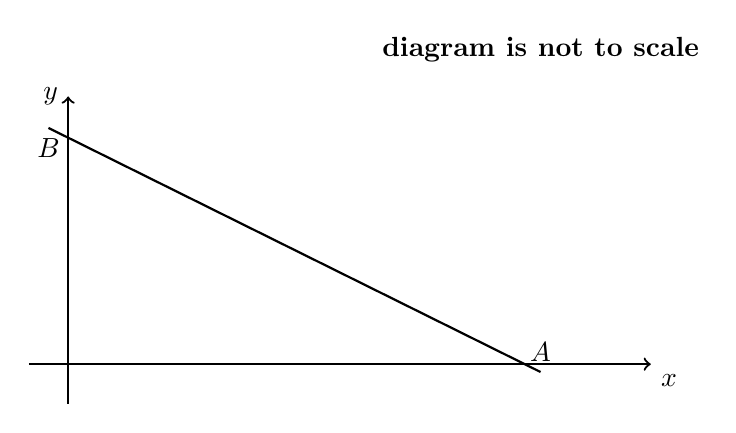
\begin{tikzpicture}[scale=1]
            %\draw [help lines] (0,0) grid (10,8);
            \draw [thick, ->] (-0.5,0) -- (7.4,0) node [below right] {$x$};
            \draw [thick, ->] (0,-0.5)--(0,3.4) node [left] {$y$};
            %\draw [fill] (9,5) circle [radius=0.1];
            \draw [thick, -] (-0.25,3) node [below] {$B$}--(6,-0.1) node [above] {$A$};
            \node at (6,4){\textbf{diagram is not to scale}};
            \end{tikzpicture}
        \end{center}
        The gradient of $L_1$ is $-\frac{3}{4}$.
        \begin{enumerate}%[itemsep=3cm]
            \item Write down the equation of the line $L_1$. \hfill [1]
            \item Find the value of $k$. \hfill [2]
            \item The line $L_2$ is perpendicular to $L_1$ and passes through $(2,1)$.
                \begin{enumerate}
                    \item Write down the gradient of the line $L_2$. \hfill [1]
                    \item Hence, write down the equation of $L_2$. Leave your answer in the form \\ $y-a=m(x-b)$. \hfill [2]
                \end{enumerate}
        \end{enumerate}
        \begin{tikzpicture}
            \draw (0,3) rectangle (15,11);
            \draw [dotted] (1,10)--(14,10);
            \draw [dotted] (1,9)--(14,9);
            \draw [dotted] (1,8)--(14,8);
            \draw [dotted] (1,7)--(14,7);
        \end{tikzpicture}

\newpage 
    \item {[Maximum mark: 7]} \\[0.3cm]
    Let $f(x)=2x+8$ and $g(x)=\sqrt{x}-1$, for $x \geq 0$.
        \begin{enumerate}
            \item Write down $g(9)$. \hfill [1]
            \item Find $(f - g)(x)$. \hfill [1]
            \item Find $(g \circ f)(4)$. \hfill [1]
            \item Write down $g^{-1}(4)$. \hfill [2]
            \item Find $f^{-1}(x)$. \hfill [2]
        \end{enumerate}
        \begin{tikzpicture}

            \draw (0,0) rectangle (15.2,15);
            \draw (8,0) rectangle (15.2,5);
            \node at (0,15)[below right]{\textbf{Working:}};
            \node at (8,5)[below right]{\textbf{Answers:}};
            \draw [dotted] (9,3.8)node[left]{(a)}--(15,3.8);
            \draw [dotted] (9,3.1)node[left]{(b)}--(15,3.1);
            \draw [dotted] (9,2.4)node[left]{(c)}--(15,2.4);
            \draw [dotted] (9,1.7)node[left]{(d)}--(15,1.7);
            \draw [dotted] (9,1)node[left]{(e)}--(15,1);
        \end{tikzpicture}

\newpage
   \item {[Maximum mark: 6]} \\[0.3cm]
   Early finishers: The diagram below shows the graph of a function $f$ for $-2 \leq x \leq 2.5$. 
        \begin{center}
        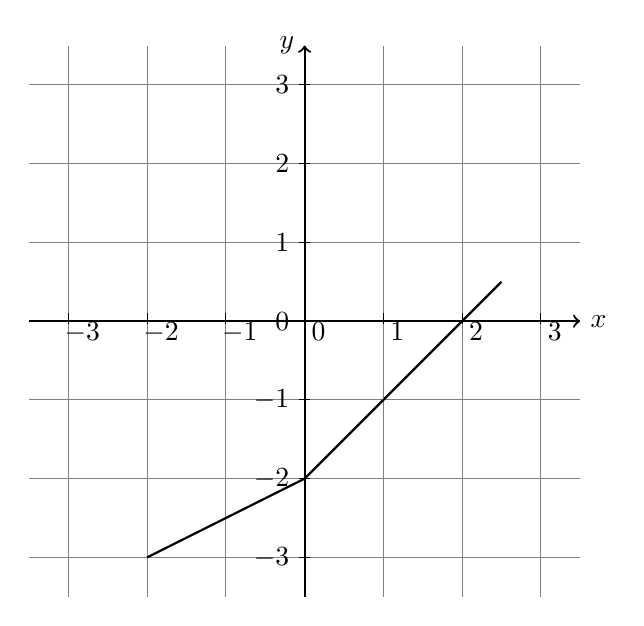
\begin{tikzpicture}[scale=1.0]
                \draw [thin, color=gray, xstep=1.0cm,ystep=1.0cm] (-3.5,-3.5) grid (3.5,3.5);
                %\draw [thin, color=lightgray,, xstep=0.2cm,ystep=0.2cm] (-5.5,-4.5) grid (5.5,6.5);
                \foreach \x in {-3, -2, -1, 0,1,2,3}
                    \draw[shift={(\x,0)},color=black] (0pt,-1pt) -- (0pt,3pt) node[below]  {$\quad \x$};
                \foreach \y in {-3, -2,-1,0,1,2,3}
                    \draw[shift={(0,\y)},color=black] (2pt,0pt) -- (-2pt,0pt) node[left]  {$\y$};
                \draw [thick, ->] (-3.5,0) -- (+3.5,0) node [right] {$x$};
                \draw [thick, ->] (0,-3.5) -- (0,3.5) node [left] {$y$};
                \draw [thick] (0,-2)--(2.5,0.5);
                \draw [thick] (0,-2)--(-2,-3);
                %\draw [thick] plot[domain= -2:3] (\x, {-2*(-\x+3)^0.5 +2});
            %\draw [thick] plot[domain= -1:2] (\x, \x*1/2 -2);
            %\draw [thick] (-2,-2).. controls (0,-1) and (2,0) .. (3,1);
            %\draw [fill] (-3,3) circle[radius=0.1] node[above left]{$A(-3,3)$};
        \end{tikzpicture}
        \end{center}
        \begin{enumerate}%[itemsep=2cm]
            \item Write down the value of $f(2)$. \hfill [1]
            \item Write down the value of $f^{-1}(-1)$. \hfill [2]
            \item Sketch the graph of $f^{-1}$ on the grid. \hfill [3]
        \end{enumerate}
        \begin{tikzpicture}
            \draw (0,1) rectangle (15.5,11);
            \draw [dotted] (1,10)--(14,10);
            \draw [dotted] (1,9)--(14,9);
            \draw [dotted] (1,8)--(14,8);
            \draw [dotted] (1,7)--(14,7);
            \draw [dotted] (1,6)--(14,6);
        \end{tikzpicture}

\newpage
    \item  {[Maximum mark: 6]} \\[0.3cm]
        The North Carolina Research Triangle is one of the world's leading regions for high tech businesses and research. The three universities that anchor the area, Duke University, University of North Carolina at Chapel Hill, and North Carolina State University, form a triangle as shown below. \\[0.25cm]
        Assume that the distance from UNCC to NC State is 40 km, from UNCC to Duke is 16 km, and that the angle made by Duke, UNCC, and NC State is $64^\circ$.
        \begin{center}
        \begin{tikzpicture}[scale=1.2]
            \draw [-, thick] (40:3) node[above right]{Duke}--
            (0,0) node[left]{UNCC}--
            (-25:7) node[right]{NC State}--cycle;
            \draw (-25:0.9) arc (-25:40:0.9);
            \node at (0.2, 0.1)[right]{$64^\circ$};
            \node at (-30:4)[above left]{40 km};
            \node at (65:1.8)[below]{16 km};
        \end{tikzpicture}
        \end{center} 
        \begin{enumerate}
            \item Calculate the distance from Duke to NC State. \hfill [3]
            \item Find the area of the triangle formed by the three universities. \hfill [3]
        \end{enumerate}
        \begin{tikzpicture}
            \draw (0,0) rectangle (15.2,8);
            \draw (8,0) rectangle (15.2,3);
            \node at (0,8)[below right]{\textbf{Working:}};
            \node at (8,3)[below right]{\textbf{Answers:}};
            \draw [dotted] (9,1.7)node[left]{(a)}--(15,1.7);
            \draw [dotted] (9,1)node[left]{(b)}--(15,1);
        \end{tikzpicture}

\newpage 
    \item {[Maximum mark: 6]} \\[0.3cm]
    The following table shows the Diploma score $x$ and university entrance mark $y$ for seven IB Diploma students. 
            \begin{center}
            \begin{tabular}{|l|c|c|c|c|c|c|c|}
                \hline
                Diploma score ($x$) & 28 & 30 & 27 & 31 & 32 & 25 & 27 \\ 
                \hline 
                University entrance mark ($y$) & 73.9 & 78.1 & 70.2 & 82.2 & 85.5 & 62.7 & 69.4 \\ 
                \hline 
                \end{tabular}
            \end{center}
            \begin{enumerate}
                \item Find the correlation coefficient. \hfill [2]\\[0.25cm]
                The relationship can be modelled by the regression line with equation $y=ax+b$.
                \item Write down the value of $a$ and of $b$ \hfill [2]\\[0.25cm]
                Rita scored a total of 26 in her IB Diploma.
                \item Use your regression line to estimate Rita's university entrance mark. \hfill [2]
            \end{enumerate}
            \begin{tikzpicture}
                \draw (0,0) rectangle (15.2,9);
                \draw (8,0) rectangle (15.2,4);
                \node at (0,9)[below right]{\textbf{Working:}};
                \node at (8,4)[below right]{\textbf{Answers:}};
                \draw [dotted] (9,2.4)node[left]{(a)}--(15,2.4);
                \draw [dotted] (9,1.7)node[left]{(b)}--(15,1.7);
                \draw [dotted] (9,1)node[left]{(c)}--(15,1);
            \end{tikzpicture}
\newpage
    \item The chart shows the time $t$ in minutes for 60 marines to complete an obstacle course.

    \begin{center}
        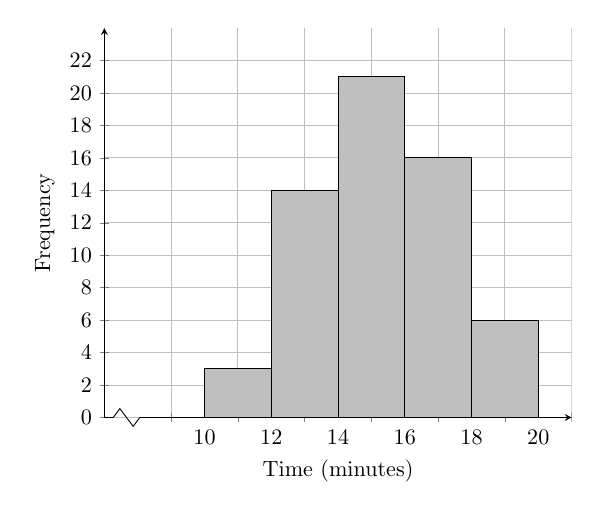
\begin{tikzpicture}[scale=0.8]
        \begin{axis}[
        xlabel=Time (minutes),
        ylabel=Frequency,
        ybar interval=1,
        xmin=8, xmax=22,
        ymin=0, ymax=24,
        xtick={10,12,14,16,18,20,22},
        ytick={0,2,4,6,8,10,12,14,16,18,20,22},
        axis lines = left,
        ymajorgrids=true,
        axis x discontinuity=crunch,
        ]
        \addplot+ [color=black, fill=lightgray]
        coordinates {(11,3) (13,14)
            (15,21) (17,16) 
            (19,6) 
            (21,3)}; %Last pair does not show
        \end{axis}
        \end{tikzpicture}
    \end{center}

    The following is the frequency table for the distribution of $t$. \\[0.25cm]
        \begin{tabular}{|l|c|c|c|c|c|}
        \hline
        Time ($t$) & $10 \leq t < 12$ & $12 \leq t < 14$ & $14 \leq t < 16$ & $16 \leq t < 18$ & $18 \leq t < 20$ \\ 
        \hline 
        Freq & 3 & 14 & 21 & $p$ & 6  \\ 
        \hline 
        \end{tabular}
        \begin{enumerate}
        \item Write down the value of $p$. \hfill [1]
        \item Write down the modal class. \hfill [1]
        \item A marine is selected at random. Find the probability that the marine completed the course in less than 14 minutes. \hfill [2]
        \item Write down the mid-interval value for the class $18 \leq t < 20$. \hfill [1]
        \item Hence find an estimate for the
        \begin{enumerate}
            \item mean; \hfill [2]
            \item standard deviation. \hfill [2] 
        \end{enumerate}
        \end{enumerate}
        \begin{tikzpicture}
            \draw (0,5) rectangle (15.5,11);
            \draw [dotted] (1,10)--(14,10);
            \draw [dotted] (1,9)--(14,9);
            \draw [dotted] (1,8)--(14,8);
            \draw [dotted] (1,7)--(14,7);
            \draw [dotted] (1,6)--(14,6);
        \end{tikzpicture}
                    
\end{enumerate}
\end{document}